\chapter{Yardım Almak}
\label{chap:bolum5}
\paragraph{Amaçlar}
\begin{itemize}
 \item Kılavuz ve bilgi sayfalarıyla çalışabilmek
 \item Nasıl Yapılır kısmını anlamak ve onları bulabilmek
 \item Diğer en önemli bilgi kaynaklarına aşina olmak
 \end{itemize}
\paragraph{Önceden Bilinmesi Gerekenler}
\begin{itemize}
 \item Linux'a Genel Bakış
 \item Temel Linux komut satırı kullanımı (örneğin daha önceki bölümlerde bahsedilenler)
\end{itemize}
\begin{section}{Kendi kendine yardım}

Linux güçlü ve karışık bir sistemdir ve kural olarak da güçlü ve karışık sistemler karmaşıktır. Belgeler, bu karmaşıklığı yönetebilmek için önemli bir araçtır. Linux'ün birçok kısmı (ne yazık ki hepsi değil) geniş olarak belgelenmiştir. Bu bölüm bu belgelere nasıl ulaşılacağının bazı yötemlerini açıklar.

Linux'ta "Yardım" birçok durumda "kendi kendine yardım" anlamına gelir. Özgür Yazılımın kültürü toplulukta boş zamanlarını geçiren diğer insanların zamanını ve iyi niyetini kılavuzun ilk birkaç paragrafında zaten açık olarak anlatılmış olan şeyleri sormamanıza dikkat çeker. Linux kullanıcısı olarak en azından mevcut belgelendirmelerin genel bilgisini edinmede ve acil durumlarda yardım almak için yapılacakları bulmada iyisinizdir. Eğer size düşeni yaparsanız göreceksiniz ki genellikle insanlar çikmazdan kurtulmanız için yardım edeceklerdir. Ama baskalarının onların yerine işlerini yapmasını bekleyen tembel bireyler hoşgörüyle karşılanmazlar.

İyice araştırılmamış sorularınıza ve problemlerinize haftanın yedi günü birinin cevap vermesini istiyorsanız çok sayıda bulunan "ticari" destek tekliflerinden faydalanmanız gerekir. Bunlar bütün ortak dağıtımlar için mevcut olup bu destek ya dağıtım satıcısı tarafından ya da yan şirketlerle verilmektedir. Farklı servis satıcılarını karşılaştırın, hangisinin fiyatı ve servis anlaşması size uyuyorsa seçin.
\end{section}
\begin{section}{\emph{help} Komutu ve \emph{--help} Seçeneği}

\begin{em}bash\end{em} içerisinde dahili komutlar hakkındaki daha detaylı bilgi \emph{help} komutuna bağımsız değişken olarak komutun adı verilerek öğrenilebilir:
\begin{verbatim}
$ help exit
exit: exit [n]
    Exit the shell with a status of N.
    If N is omitted, the exit status
    is that of the last command executed.
$ _
\end{verbatim}

Daha detaylı açıklama için kabuğun rehber sayfasında ve bilgi belgelerinde mevcuttur. Bu bilgi kaynakları daha sonra bu bölümde ele alınacaktır.

Bunun yerine harici komutların (programların) birçoğu \emph{--help} seçeneğini destekler. Çoğu komut kısaca kendileriyle kullanılan parametrelerini ve sözdizminlerini sıralar.

Her komut --help seçeneğini desteklemeyebilir; sık sık çağrılan seçenekler -h veya -?, ya da yanlış bir seçenek veya geçersiz komut satırı belirtirseniz yardım ekrana gelecektir. Ne yazık ki genel kuralı yoktur.
\end{section}
\begin{section}{Çevrim İçi Kılavuz}
\begin{subsection}{Genel Bakış}

Nerdeyse her komut satırı programı ayar dosyaları ve sistem çağrıları vs. yanında "kılavuz sayfası" (ya da "man sayfası") ile gelir. Bu metinler genelde yazılımla beraber kurulur ve ,ncelemek için "\emph{man $<$isim$>$}" komutu kullanılır.

\paragraph{}{
\begin {table}[H]
\caption {Kılavuz sayfasının bölümleri} \label{tab:title} 
\begin{tabular}{c l @{} l}
\hline
Bölüm &
\multicolumn{2}{c}{İçerik} \\
\hline
NAME 	&	Komutun adı ve kısa açıklama \\
SYNOPSIS &	Komutun sözdizimi açıklaması \\
DESCRIPTION &	Komutun etkisi ile ilgili açıklama \\
OPTIONS &	Kullanılabilir seçenekler \\
ARGUMENTS &	Kullanılabilir bağımsız değişkenler \\
FILES 	&	Yardımcı dosyalar \\
EXAMPLES &	Örnek komut satırları \\
SEE ALSO &	İlgili konulara çapraz referanslar \\
DIAGNOSTICS &	Hata ve uyarı mesajları \\
COPYRIGHT & 	Komutun yazarları \\
BUGS	&	Bilinen komut sınırlamaları \\
\hline
\end{tabular}
\end {table}
}

Buradaki \emph{$<$isim$>$} açıklanmasını istediğiniz komutun yada dosyanın adıdır. Örneğin "\emph{man bash}", anılan iç kabuk komutlarının listesini üretir.

Ancak, kılavuz sayfalarinin bazi dezavantajlari vardir: Bu kılavuzların çoğu sadece İngilizcedir; farklı dillere çevirilenleri vardır ama tam değil. Üstelik açiklamalar çoğunlukla karışıktır. Her kelime çok önemlidir, bu durum da yeni başlayanlar için belgeleri erişilebilirlikten uzaklaştırır. Ek olarak, özellikle uzun belgelerin yapısı anlaşılmaz olabilir. Öyle olsa bile, bu belgelerin değeri göz ardı edilemez. Kağıtlarla kullanıcıyı canından bezdirmek yerine sistemle beraber çevrim içi kılavuz mevcuttur.

Birçok Linux dağıtımlari komut satırından çağrılabilen her komut için bir kılavuz sayfasının olması gerektiği felsefesini takip eder. Bu durum KDE ve GNOME görsel masaüstü ortamına ait programlar için aynı ölçüde geçerli değildir. Bunların pek çoğunun hiç bir kılavuz sayfasının bulunmaması yanında bazıları da görsel masaüstü çevresinde bile berbat bir şekilde belgelendirilmiştir. Bu programların çoğunun gönüllüler tarafından katkıda bulunulduğu gerçegi sadece zayıf bir bahanedir.
\end{subsection}
\begin{subsection}{Yapı}

Yardım sayfalarının yapısı kabaca Tablo 5.1 taslağını takip eder. Yine de her kılavuz sayfası orada belirtilen her bölümü içermeyebilir. Özellikle de, EXAMPLES kısmı sık sık kısa kısa verilmiştir.

BUGS başlığı genellikle yanlış anlaşılır: Düzeltilen uygulamanın içindeki \emph{hataları} okuyun; elbette burada belgelendirilen genellikle komutun aldığı yaklaşımdaki kısıtlamalardır ve siz bu kısıtlamaların makul bir çabayla kaldırılamadığını bir kullanıcı olarak bilmelisiniz. Örneğin, \emph{grep} komutunun belgeleri düzenli ifadelerin çeşitli yapılarının bulunması grep sürecinin çok bellek kullanmasına yol açabildiğini belirtir. Bu \emph{grep} komutunun uyguladığı arama yönteminin sonucudur ve önemsiz, kolayca giderilebilen hata değildir.    

Yardım sayfaları \emph{groff} adında bir program tarafından metni görüntülemek veya yazdırmak için özel bir girdi biçimi olarak yazılır. Kılavuz sayfaları /usr/share/man dizininin \emph{man}n alt dizini içinde saklanır. n Tablo 5.2'de verilen bölüm numaraları içindir.

Diğer dizinlerdeki yardım sayfalarını, \emph{man} komutu tarafından sırasıyla taranacak dizinleri içeren, MANPATH çevresel değişkenini ayarlayarak birleştirebilirsiniz. \emph{manpath} komutu MANPATH değişkeninin nasıl ayarlanabileceği hakkında ipuçları barındırır.
\paragraph{}{
\begin {table}[H]
\caption {Kılavuz sayfası konuları} \label{tab:title} 
\begin{tabular}{c l @{} l}
\hline
Bölüm &
\multicolumn{2}{c}{İçerik} \\
\hline
1 	&	Kullanıcı komutları \\
2 &	Sistem çağrıları \\
3 &	C dili kütüphane işlevleri \\
4 &	Aygıt dosyaları ve sürücüleri \\
5 &	Ayar dosyaları ve dosya formatları \\
6 & Oyunlar \\
7 &	Çeşitli (örneğin groff makroları, ASCII tabloları, …) \\
8 &	Yönetici komutları \\
9 &	Çekirdek işlevleri \\
n & "Yeni" komutlar \\
\hline
\end{tabular}
\end {table}
}
\end{subsection}
\begin{subsection}{Bölümler}

Her kılavuz sayfası "kılavuzu" kapsayan "bölüme" aittir (Tablo 5.2). 1., 5. ve 8. bölümler en önemlileridir. Aramayı daraltmak için \emph{man} komutu satırına bölüm numarası verebilirsiniz. Örneğin, "\emph{man 1 crontab}" \emph{crontab} komutu için kılavuz sayfasını görüntülerken, "\emph{man 5 crontab}"-\emph{crontab} dosyalarının biçimlerini açıklar. Kılavuz sayfalarını işaret ederken, bölüm numarasını parantez içinde belirtmek gelenekseldir; biz, \emph{crontab}(1) \emph{crontab} komut kılavuzu, ve \emph{crontab}(5) dosya biçimi açıklaması aradaki farkı ayırt ederiz.

-a seçeneğiyle \emph{man} verilen isme göre bulunan kılavuzu gösterir; seçenek vermezsek ilk bulunan sayfayı (genellikle bölüm 1) gösterir.
\end{subsection}
\begin{subsection}{Kılavuz Sayfalarını Görüntülemek}

Kılavuz sayfalarını metin terminalde görüntülemek daha üzerinde duracağımız \emph{less} ile gerçekleştirilir. Bu aşamada kılavuz sayfasında yukarı ok \begin{math}\uparrow\end{math} ve aşağı ok \begin{math}\downarrow\end{math} tuşları ile gezinebileceğinizi bilmek önemlidir. Metnin içindeki bir anahtar kelimeyi \emph{/} tuşuna basıp ardından kelimeyi girip Enter tuşuna basarak arayabilirsiniz. Her geri dönüş tuşuna bastığınızda bir sonraki bulunan kayda sıçrar (eğer varsa). Kabuğa \emph{q} tusuna basarak geri dönebilirsiniz.

KDE web tarayıcısı, Konqueror, kullanarak güzel biçimlendirilmiş uygun kılavuz sayfaları elde etmek mümkündür. Basitçe "\emph{man:/$<$isim$>$}" (hatta "\emph{\#$<$isim$>$}") URL adresini tarayıcının adres satırına girin. Bu yöntem aynı zamanda KDE komut satırı için de geçerlidir.

\begin{figure}
        \centering
        \begin{subfigure}[b]{0.3\textwidth}
                \centering
                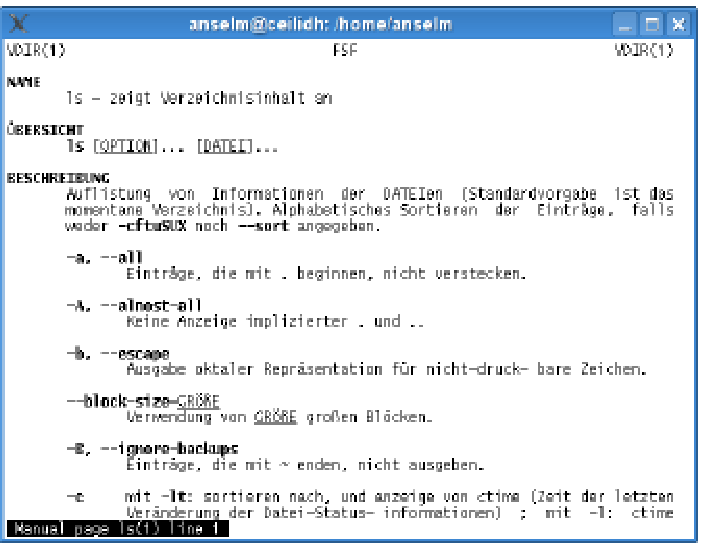
\includegraphics[width=\textwidth]{./bolum5/img1}
        \end{subfigure}%
        ~ %add desired spacing between images, e. g. ~, \quad, \qquad etc. 
          %(or a blank line to force the subfigure onto a new line)
        \begin{subfigure}[b]{0.3\textwidth}
                \centering
                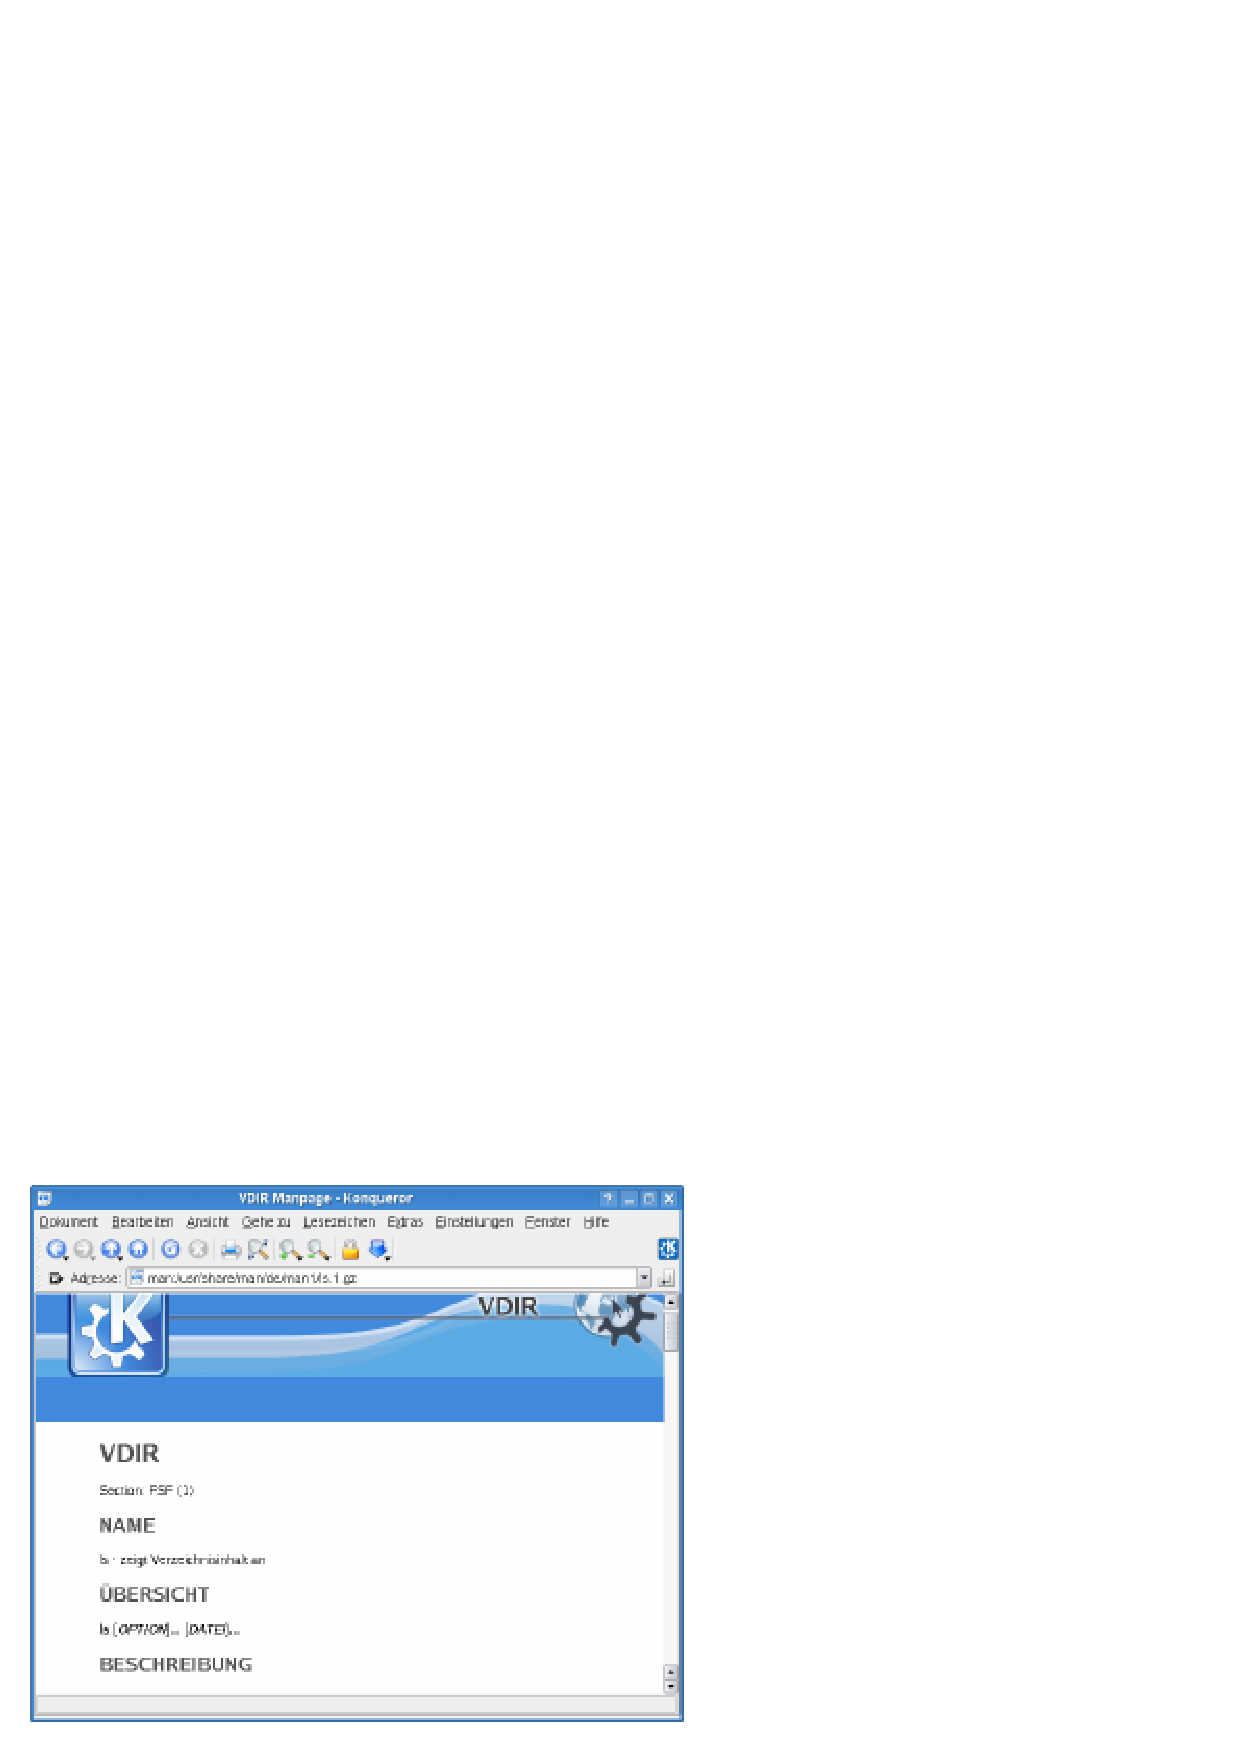
\includegraphics[width=\textwidth]{./bolum5/img2}
        \end{subfigure}
        \caption{Metin terminali (sol) ve Konqueror (sağ) içerisinde bir kılavuz sayfası }\label{fig:manpages}
\end{figure}

Amaçsızca sayısız kılavuz sayfasını aramadan önce, konu hakkında \emph{apropos} yardımıyla genel bir bilgi edinmek daha mantıklıdır. Bu komut basitçe şöyle çalıştırılır "man -k"; her ikisi de komut satırında verilen bir anahtar kelimenin "NAME" bölümlerine ilişkin tüm kılavuz sayfalarını arar. Bunun sonucunun çıktısı tüm man sayfalarını, adı veya açıklama kısmında anahtar kelimeyi de içerecek şekilde bir liste görüntüler.

Bu konuyla alakalı olan bir başka komut \emph{whatis} komutudur.Bu komut da tüm man sayfalarını arar ama yukarıda belirttiğimiz komuttan farkı \emph{whatis} aramayı anahtar kelimeye göre değil de komutun (dosya,...) \emph{adına} göre yapar. Bu istenilen komut, sistem çağrıları vs. hakkında kısaca bir açıklama görüntüler. Özellikle söz konusu man sayfasının(lar) "NAME" bölümünün ikinci  kısmını verir. \emph{whatis} ile "man -f" eşdeğerdir.
\paragraph{Alıştırmalar}{
\begin{itemize}
 \item \emph{ls} komutu için kılavuz sayfasını görüntüleyin. Metin tabanlı \emph{man} komutunu kullanın ve eğer mümkünse - Konqueror tarayıcısını da kullanın.
 \item Sisteminizde hangi kılavuz sayfaları (en azından "NAME" bölümlerine göre) süreçlerle iş yapar.
 \item (Ileri düzey) Kuramsal bir komutun kılavuz sayfasını yazmak için metin editörü kullanın. Önceden \emph{man}(7) kılavuz sayfasını okuyun. Kılavuz sayfasının görünürlüğünü hem ekranda ("\emph{groff -Tascii -man $<$dosya$>$ | less}" komutunu kullanarak) hem de yazılı çıktı olarak ("\emph{groff -Tps -man $<$dosya$>$ | gv -}" gibi birşey kullanın) kontrol edin.
\end{itemize}}
\end{subsection}
\end{section}
\begin{section}{Bilgi Sayfaları}

Bazı komutlar için - genellikle karmaşık olanlar için sıradan kılavuz sayfaları yerine (ya da ilave olarak) "bilgi sayfaları" mevcuttur. Bunlar genellikle daha geniş olup World Wide Web'e benzer şekilde hiper metin prensibine göre kurulmuştur.

Bilgi sayfaları fikri GNU projesi ile birlikte ortaya çıkmıştır; o yüzden onlar en sık FSF (Özgür Yazılım Vakfı) ile  yayımlanan veya GNU projesine ait yazılımlarla gelir. Aslında "GNU sistem" için sadece bilgi belgeleri olması gerekiyordu; ancak GNU, FSF himayesinde geliştirilmeyen bir sürü yazılımları da kendi içine alır, ve GNU araçları çizgileri daha kesin olan sistemlerde kullanıldığından FSF bazı durumlarda taviz vermeye başladı.

Kılavuz sayfalarının dengi olan bilgi sayfaları "\emph{info $<$komut$>$}" komutu (bilgi programını içeren paket açıkça kurulmuş olması gerekebilir) kullanılarak görüntülenir. Ayrıca, bilgi sayfaları \emph{emacs} editöründe veya KDE web tarayıcısı Konqueror'da URL'ler yardımıyla "\emph{info:/$<$komut$>$}" görüntülenebilir.

Bilgi sayfalarının bir avantajı, kılavuz sayfaları gibi kaynak formatında yazılmış olmalarıdır. Bilgi sayfaları PDF ve PostScript formatında yazdırılabilir veya ekranda işlenebilir. \emph{groff} yerine, \TeX{} dizgi programı çıktı işlemi için hazırlanabilir.

\paragraph{Alıştırmalar}{
\begin{itemize}
 \item \emph{ls} programı için bilgi sayfasına bakın. Metin tabanlı bilgi tarayıcısı ve, varsa, Konqueror tarayıcısını deneyin.
 \item Bilgi sayfaları günümüzde HTML dosyalarının World Wide Web'de olduğu gibi hiper metnin ilkel formunu kullanır. Bilgi sayfaları neden HTML ile yazılmamıştır?
\end{itemize}}
\end{section}
\begin{section}{NASIL Belgeleri}

Kılavuz ile bilgi sayfaları arasındaki ortak problem şudur: Kullanıcılar kullanacakları programın adını bilmek zorundadırlar. Hatta \emph{apropos} ile arama yapmak şans oyunu gibi birşeydir. Ayrıca, her problem tek bir komut kullanılarak çözülemez. Bu nedenle bunlar "komut odaklı" belgeler yerine genellikle "problem odaklı" olarak adlandırılır. Nasıl Yapılır kısmı bunlara çözüm üretmek için tasarlandı.

Nasıl Belgeleri kendilerini tek bir komutla  kısıtlamayan geniş kapsamlı belgelerdir, ama sorunların çözümü için tam yaklaşımları açıklamaya çalışırlar. Örneğin, DSL yoluyla Linux sisteminin internete nasıl bağlanacağını detaylı olarak açıklayan "DSL Nasıl" belgesi vardır, ya da Linux için astronomi yazılımını tartışan "Astronomi NASIL" vardır. Nasıl Yapılır kısımlarının birçoğu İnglizce aslını genellikle geriden takip etse de bunlar başka dillerde de mevcuttur.

Çoğu Linux dağıtımı Nasıl Belgelerinin (veya büyük bir alt kümesinin) yerel olarak kurulu olmasını sağlar. Bunlar dağıtıma özel dizinlerin altında bulunurlar. /usr/share/doc/howto SUSE dağıtımları için, /usr/share/HOWTO Debian GNU/Linux içindir. Tipik olarak düz metin veya HTML dosyaları içerir. Nasıl Yapılır'ların geçerli tüm sürümleri ve diğer PostScript veya PDF biçimindekilerinin hepsi internet üzerinde "Linux Belgelendirme Projesi" (http://www.tldp.org) altında bulunabilir. Bu adres ayrıca diğer Linux belgelerini de sunar.
\end{section}
\begin{section}{Ek Bilgi Kaynakları}

Neredeyse her kurulu olan yazılım için ilave belgeleri veya örnek dosyaları /usr/share/doc ya da /usr/share/doc/packages (kullandığınız dağıtıma bağlı olarak değişir) altında bulunur. Çoğu GUI uygulamaları (KDE veya GNOME paketlerindeki gibi) "yardım" menüsü sunar. Üstelik birçok dağıtım uzmanlaştırılmış "yardım merkezleri" sunar. Sistem üzerindeki çoğu belgelere uygun erişimi sağlar.

Yerel sistemden bağımsız olarak WWW ve USENET arşivlerinin de arasında bulunduğu, pek çok belge Internet ortamında bulunmaktadır. 

Linux için daha ilgi çekici sitelerden bazıları:
\paragraph{http://www.tldp.org/}{“Linux Belgelendirme Projesi”, kılavuz sayfaları ve Nasıl Yapılır'dan sorumlu (diğer şeylerin yanı sıra).}
\paragraph{http://www.linux.org/}{Linux meraklıları için genel portal.}
\paragraph{http://www.linuxwiki.de/}{Linux ile ilgili her şey için serbest biçimli metin bilgi veritabanı (Almanca)}
\paragraph{http://lwn.net/}{Haftalık Linux Haberleri - her türlü Linux haberleri için belki de en iyi web sitesi. Yeni gelişmeler, ürünler, güvenlik açıkları, basındaki Linux savunuculuğu vs. ayrıca her persembe günü geçmiş haftaların araştırmalarının yer aldığı çevrimiçi dergi de bulunur. Günlük haberlere ücretsiz olarak ulaşılabilir iken haftalık yayınlamalara belli bir ücret ödenmesi gerekiyor (aylık 5\$'dan başlayan fiyatlarla). İlk çıktığı haftadan sonra o yayınları ücretsiz olarak erişilebilir hale getiriyorlar.}
\paragraph{http://freecode.com/}{Bu site yeni (genel olarak serbest) çıkan yazılım paketlerini tanıtır. Buna ek olarak ilginç projeler veya yazılım paketleri için sorguları sağlayan bir veritabanı var}
\paragraph{http://www.linux-knowledge-portal.de/}{LWN ve Freshmeat dahil diğer Linux sitelerinden haber başlıklarını toplar.}

Eğer Internette veya Usenet arşivlerinde bulmadıysanız aradığınızı, sorunuza cevabı  posta listelerinde ya da Usenet gruplarında soru sormak her zaman mümkündür. Bu forumlardaki çoğu kullanıcıların daha önce cevaplanmış ya da belgelendirmede veya "SSS" (Sıkça Sorulan Sorula) kısmında olan birşeyi sormanıza kötü tepki verebileceklerini unutmayın. Probleminizin detaylı açıklamasını hazırlayın, kayıt dosyalarından ilgili ayrıntıları verin çünkü karmaşık problemleri sizde olduğu gibi uzak mesafeden çözmek zordur (karmaşık olmayan problemleri kendinizin çözebiliyor olmanız lazım).

Haber arşivlerini \emph{http://groups.google.com/} (eskiden DejaNews) adresinde bulabilirsiniz.

Linux için ilgi çekici \emph{haber grupları} İngilizce için \emph{comp.os.linux.*} veya Almanca için \emph{de.comp.os.linux.*} hiyerarşilerinde bulunabilir. Birçok Unix grupları Linux konuları için uygundur; kabukla ilgili soruların kabuk programlama için ayrılan grupta sorulması gerekir, Linux grubunda değil, çünkü kabuklar genellikle Linux'a özgü değildir.

Linux tabanlı posta listelerini örneğin, \emph{majordomo@vger.kernel.org} adresinde bulabilirsiniz. LIST denilen listeye katılmak için önce "subscribe LIST" adresine e-posta atmanız gerekir. Sistemde mevcut yorumlanmış tüm posta listeleri \emph{http://vger.kernel.org/vger-lists.html} adresinde bulabilirsiniz.

Görünüşte anlaşılmayan problemleri çözmenin yolu hata mesajının Google'da aratmaktır(ya da güvendiğiniz baska bir arama motoru). Eğer faydalı bir sonuç alamazsanız, arama yaptığınız sorguda sadece size özel duruma bağlı kısımları kaldırın (mesela alan adları gibi). Google'da aramanın avantajı sadece ortak web sayfalarını indekslemek değil bunun yanında posta liste arsivlerini de indeksler. O yüzden sizin gibi sorunu yaşayan bir başka birilerinin bulunması da olası bir durum.

Açık kaynak kodlu yazılımların büyük miktarda belgelendirmelerinin olması tek büyük faydaları değildir ayrıca çoğu belgelendirmenin de en az yazılımının kendisi gibi kısıtlı olmasıdır. Bu, yazılım geliştiricileri ve belge yazarları arasındaki işbirliğini kolaylaştırır ve belgelerin diğer dillere çevrilmesi daha kolaydır. Aslında, programcı olmayanlar için özgür yazılım projelerine destek verebilmeleri için bol fırsat bulunmaktadır, örn. iyi belgelemeler yazmak. Özgür yazılım faaliyet alanında programcılara verilen saygıyı belge yazarlarına da vermeye çalışılmalı. Bu durum kaymasının başlamış olması henüz tamamlandığı anlamına gelmemektedir.
\end{section}
\paragraph{Bu Bölümdeki Komutlar}{:\\
\textbf{apropos}	NAME bölümünde verilen anahtar kelimeyi içeren tüm kılavuz sayfalarını görüntüler \\
\textbf{groff}		Gelişmiş dizgi programı \\
\textbf{help}		\emph{bash} komutları çevrim için yardımı görüntüler \\
\textbf{info}		Karakter tabanlı terminalde GNU Bilgi sayfalarını görüntüler \\
\textbf{less}		Metinleri sayfa sayfa (kılavuz sayfaları gibi) görüntüler \\
\textbf{man}		Sistem kılavuz sayfalarını görüntüler \\
\textbf{manpath}		Sistem kılavuz sayfalarının aranacağı yolu belirler \\
\textbf{whatis}		Açıklamasında verilen belirli bir anahtar kelime ile kılavuz sayfalarını bulur \\
}
\paragraph{Özet}{
\begin{itemize}
\item "\emph{help $<$komut$>$}" dahili bash komutlarını açıklar. Birçok harici komut \emph{--help} seçeneğini destekler.
\item Çoğu program kılavuz sayfalarıyla gelir. Bunlar \emph{man} komutuyla incelenebilir. \emph{apropos} verilen anahtar kelimelere göre tüm kılavuz sayfalarını arar, \emph{whatis} kılavuz sayfa isimlerine bakar.
\item Bazı programlar için bilgi sayfaları kılavuz sayfalarına bir alternatiftir.
\item Nasıl Yapılır belgeleri problem tabanlı bir belgeleme olustururlar.
\item World Wide Web ve USENET dünyasında Linux ile ilgili çok sayıda ilginç kaynaklar var.
\end{itemize}}